\section{Experiments}
To evaluate the advantages of using the above models, the models were trained on a unimodal dataset (Figure \ref{fig:err_curve_inp}). The method of inference was using MCMC sampling using the STAN \citep{stanpaperref}. 


\begin{figure}[h]
  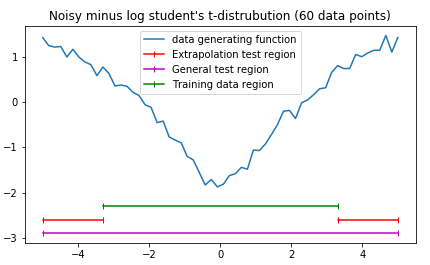
\includegraphics[scale=0.7]{err_curve_inp.png}
  \centering
  \caption{Input to the used to generate the error curve}
  \label{fig:err_curve_inp}
\end{figure}


From the error error curves of the Fig \ref{fig:err_curve} we can see that the unimodality enforced models learn much faster than normal GP regression.
\begin{figure}[h]
  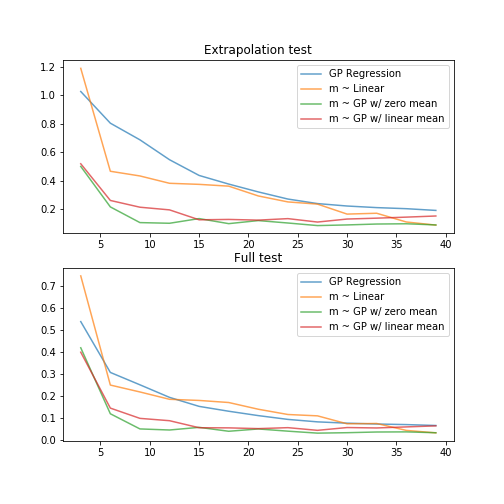
\includegraphics[scale=0.7]{err_curve.png}
  \centering
  \caption{Testing error as a function of number of data points used for training}
  \label{fig:err_curve}
\end{figure}